\documentclass[11pt]{article}
\usepackage{amsmath, amssymb}
\usepackage{geometry}
\usepackage{graphicx}
\begin{document}

\section{Introduction}
We consider as our image, the following function, defined on $[-1, 1]
\times:
[-1, 1]$
\begin{equation}\label{eq:function}
  \begin{split}
    f(x, y) &= 0.5 - 0.2x - 0.3y - 0.05x^2 + 0.03xy + 0.04y^2 \\ 
    &+ 0.03y^3 + 0.001x^3 - 0.0015x^2y + 0.002xy^2 - 0.0005y^3.
  \end{split}
\end{equation}
This function was chosen to have no critical points, and to be
predominantly linear, so that the higher order derivatives were not too
large. This was predominantly so the higher order terms in the signatures
would not overwhelm the smaller terms. The function is depicted as a
greyscale image in Figure~\ref{fig:function}
\begin{figure}
  \centering
  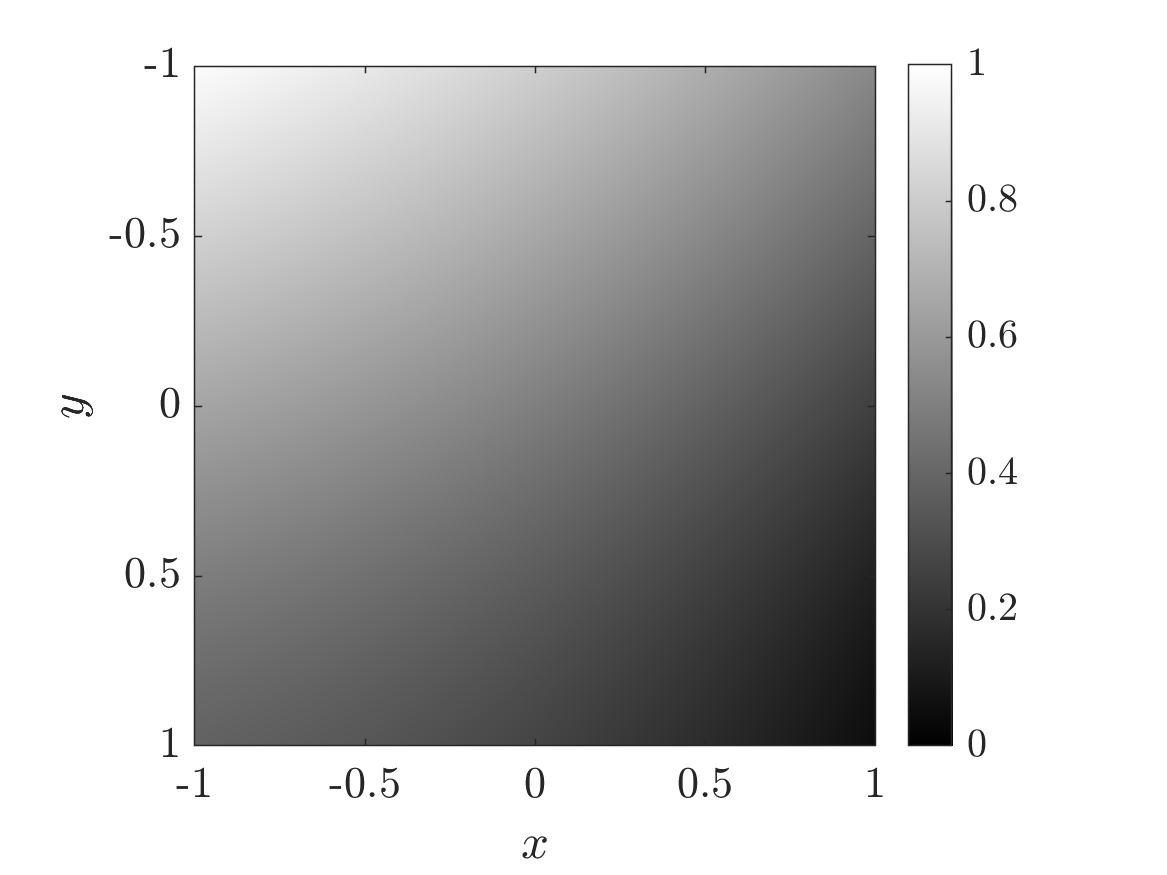
\includegraphics[width=12cm]{figures/function}
  \caption{The test function used in this document, from
  Eq.~\eqref{eq:function}.}\label{fig:function}
\end{figure}

We consider the signatures of this function under various transformation
groups, as detailed throughout the main body of the paper and illustrate
the signature in three dimensions. A grid is overlaid on the image of the
function itself, as shown in Fig~\ref{fig:function_scanlines}. This grid is
mapped to the signature surface to help understand what the signature looks
like locally.
\begin{figure}
  \centering
  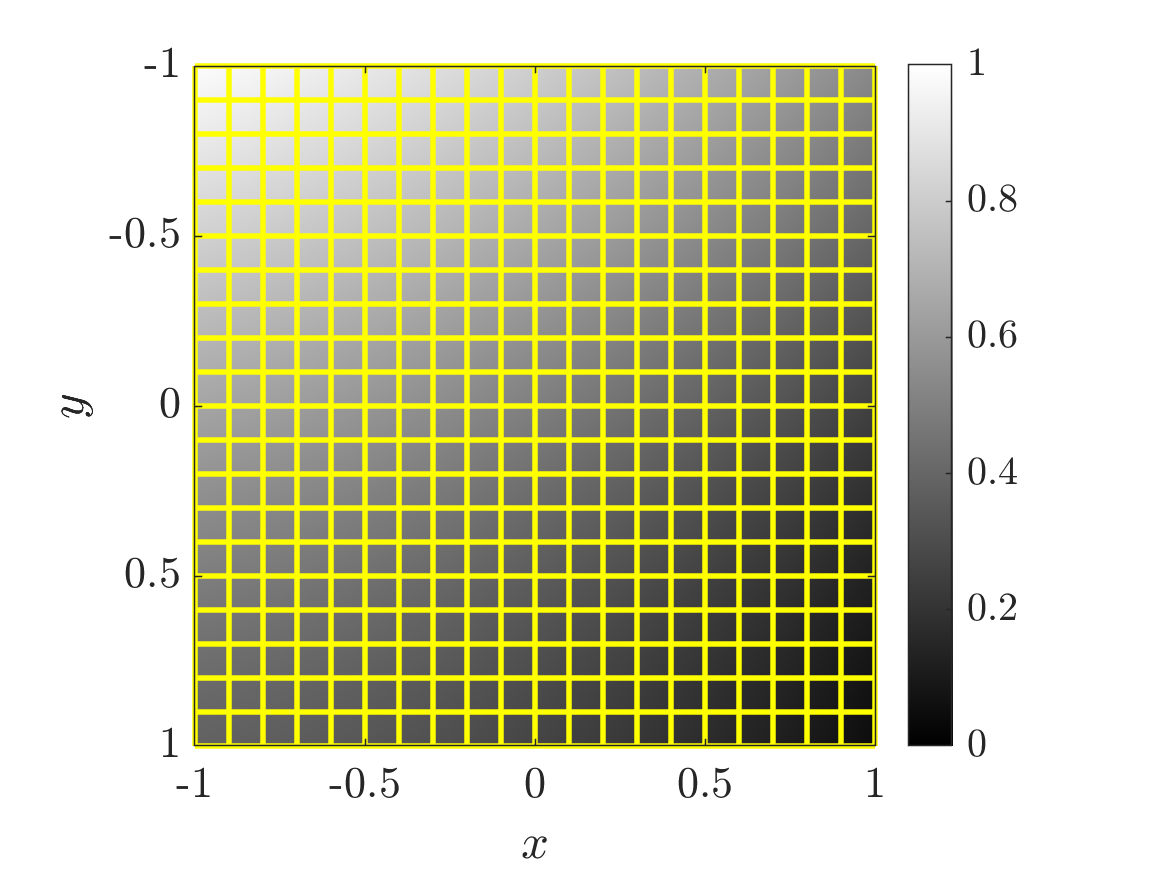
\includegraphics[width=12cm]{figures/function_scanlines}
  \caption{The test function used in this document, from
  Eq.~\eqref{eq:function} with a grid of lines
overlaid.}\label{fig:function_scanlines}
\end{figure}


\section{The transformation groups}

\subsection{Sim(2)}
For $\text{Sim}(2)$, we use the signature $(I_1, I_2, I_3)$, defined by
\begin{equation}\label{eq:sim2sig}
    I_i = \frac{f}{\sqrt{J_1^2 + J_2^2 + J_3^2}} J_i, \qquad i \in \{1, 2,
    3\}
\end{equation}
where
\begin{equation*}
  \begin{split} 
    J_1 &= f_x^2 + f_y^2, \\
    J_2 &= (f_{xx} + f_{xy})^2, \\
    J_3 &= f_{xx}^2 + 2f_{xy}^2 + f_{yy}^2.
  \end{split}
\end{equation*}
The signature is visualised in Fig.~\ref{fig:sim2signature}
\begin{figure}
  \centering
    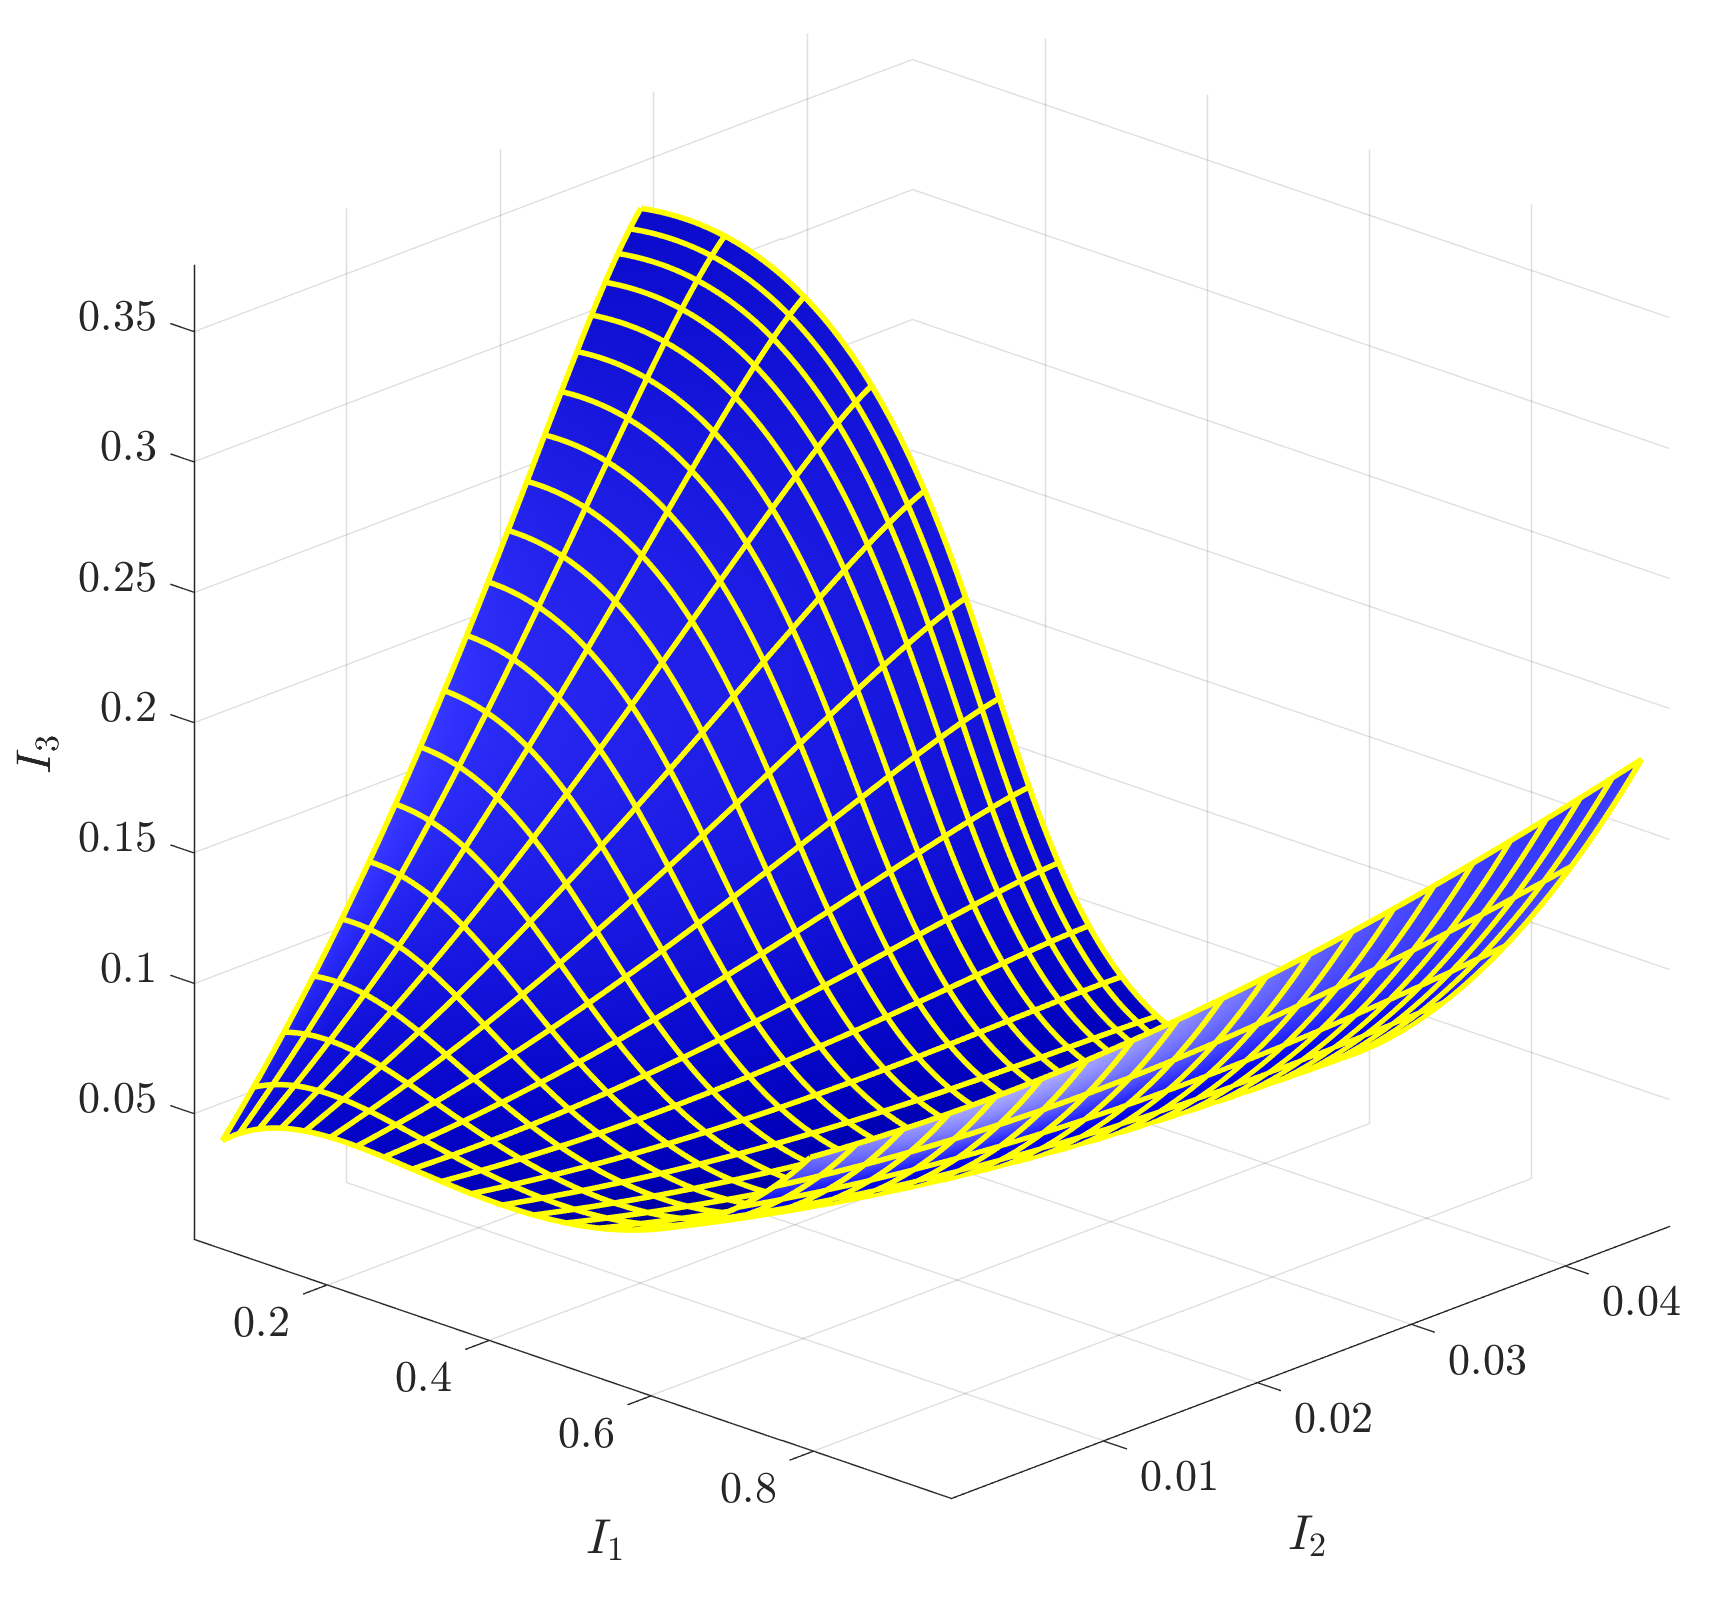
\includegraphics[width=12cm]{figures/Sim2_signature}
    \caption{$\text{Sim}(2)$ signature}
    \label{fig:sim2signature}
\end{figure}

\subsection{SE(2)}
For $SE(2)$, we use the signature
\begin{equation}\label{eq:se2sig}
  \begin{split}
    I_1 &= f \\
    I_2 &= f_x^2 + f_y^2 \\
    I_3 &= f_x^2 f_{xy} + f_x f_y f_{yy} - f_x f_y f_{xx} - f_y^2 f_{xy}
  \end{split}
\end{equation}
The signature is visualised below in Fig.~\ref{fig:se2signature}
\begin{figure}
  \centering
    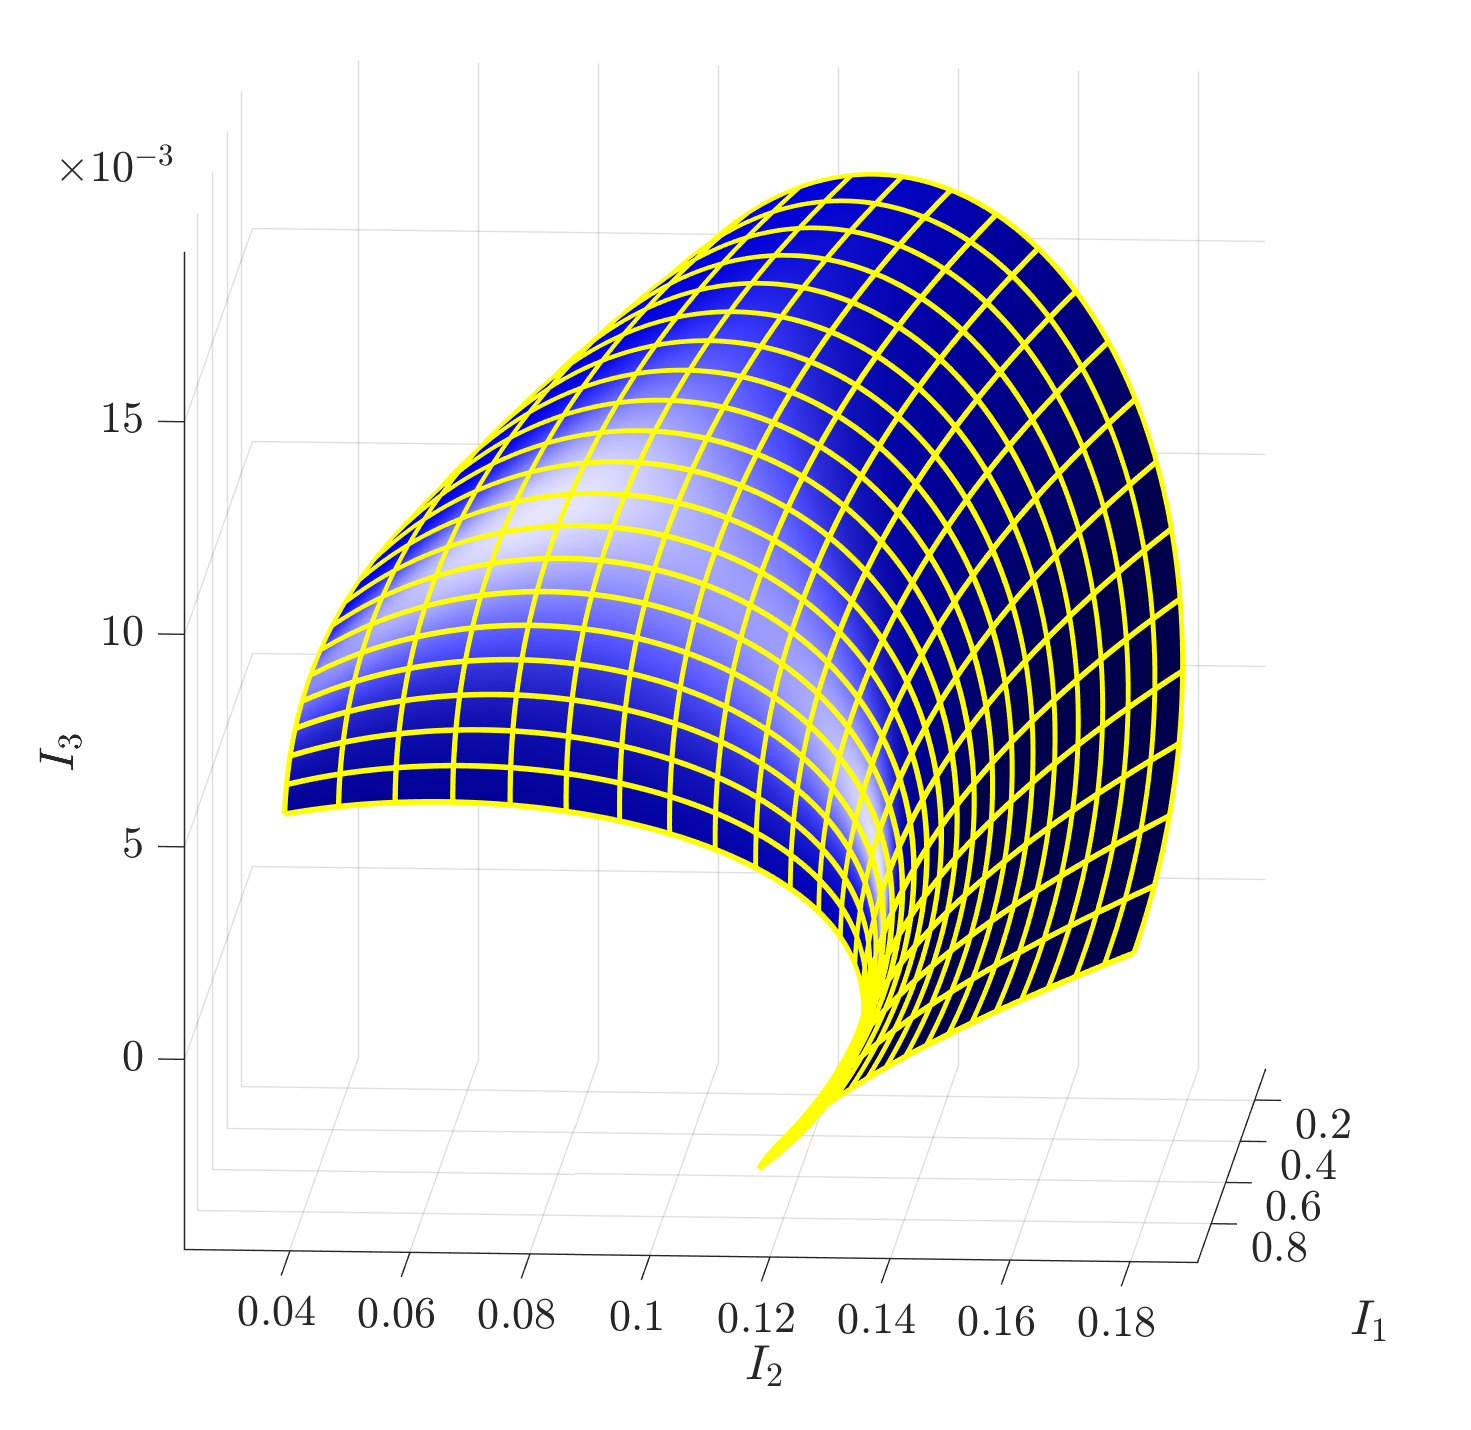
\includegraphics[width=12cm]{figures/SE2_signature}
  \caption{$SE(2)$ signature}
  \label{fig:se2signature}
\end{figure}


\subsection{E(2)}
For $E(2)$, we use the signature
\begin{equation}\label{eq:e2sig}
  \begin{split}
    I_1 &= f \\
    I_2 &= f_x^2 + f_y^2 \\
    I_3 &= f_{xx} + f_{yy}
  \end{split}
\end{equation}
The signature is visualised in Fig.~\ref{fig:e2signature}
\begin{figure}
  \centering
    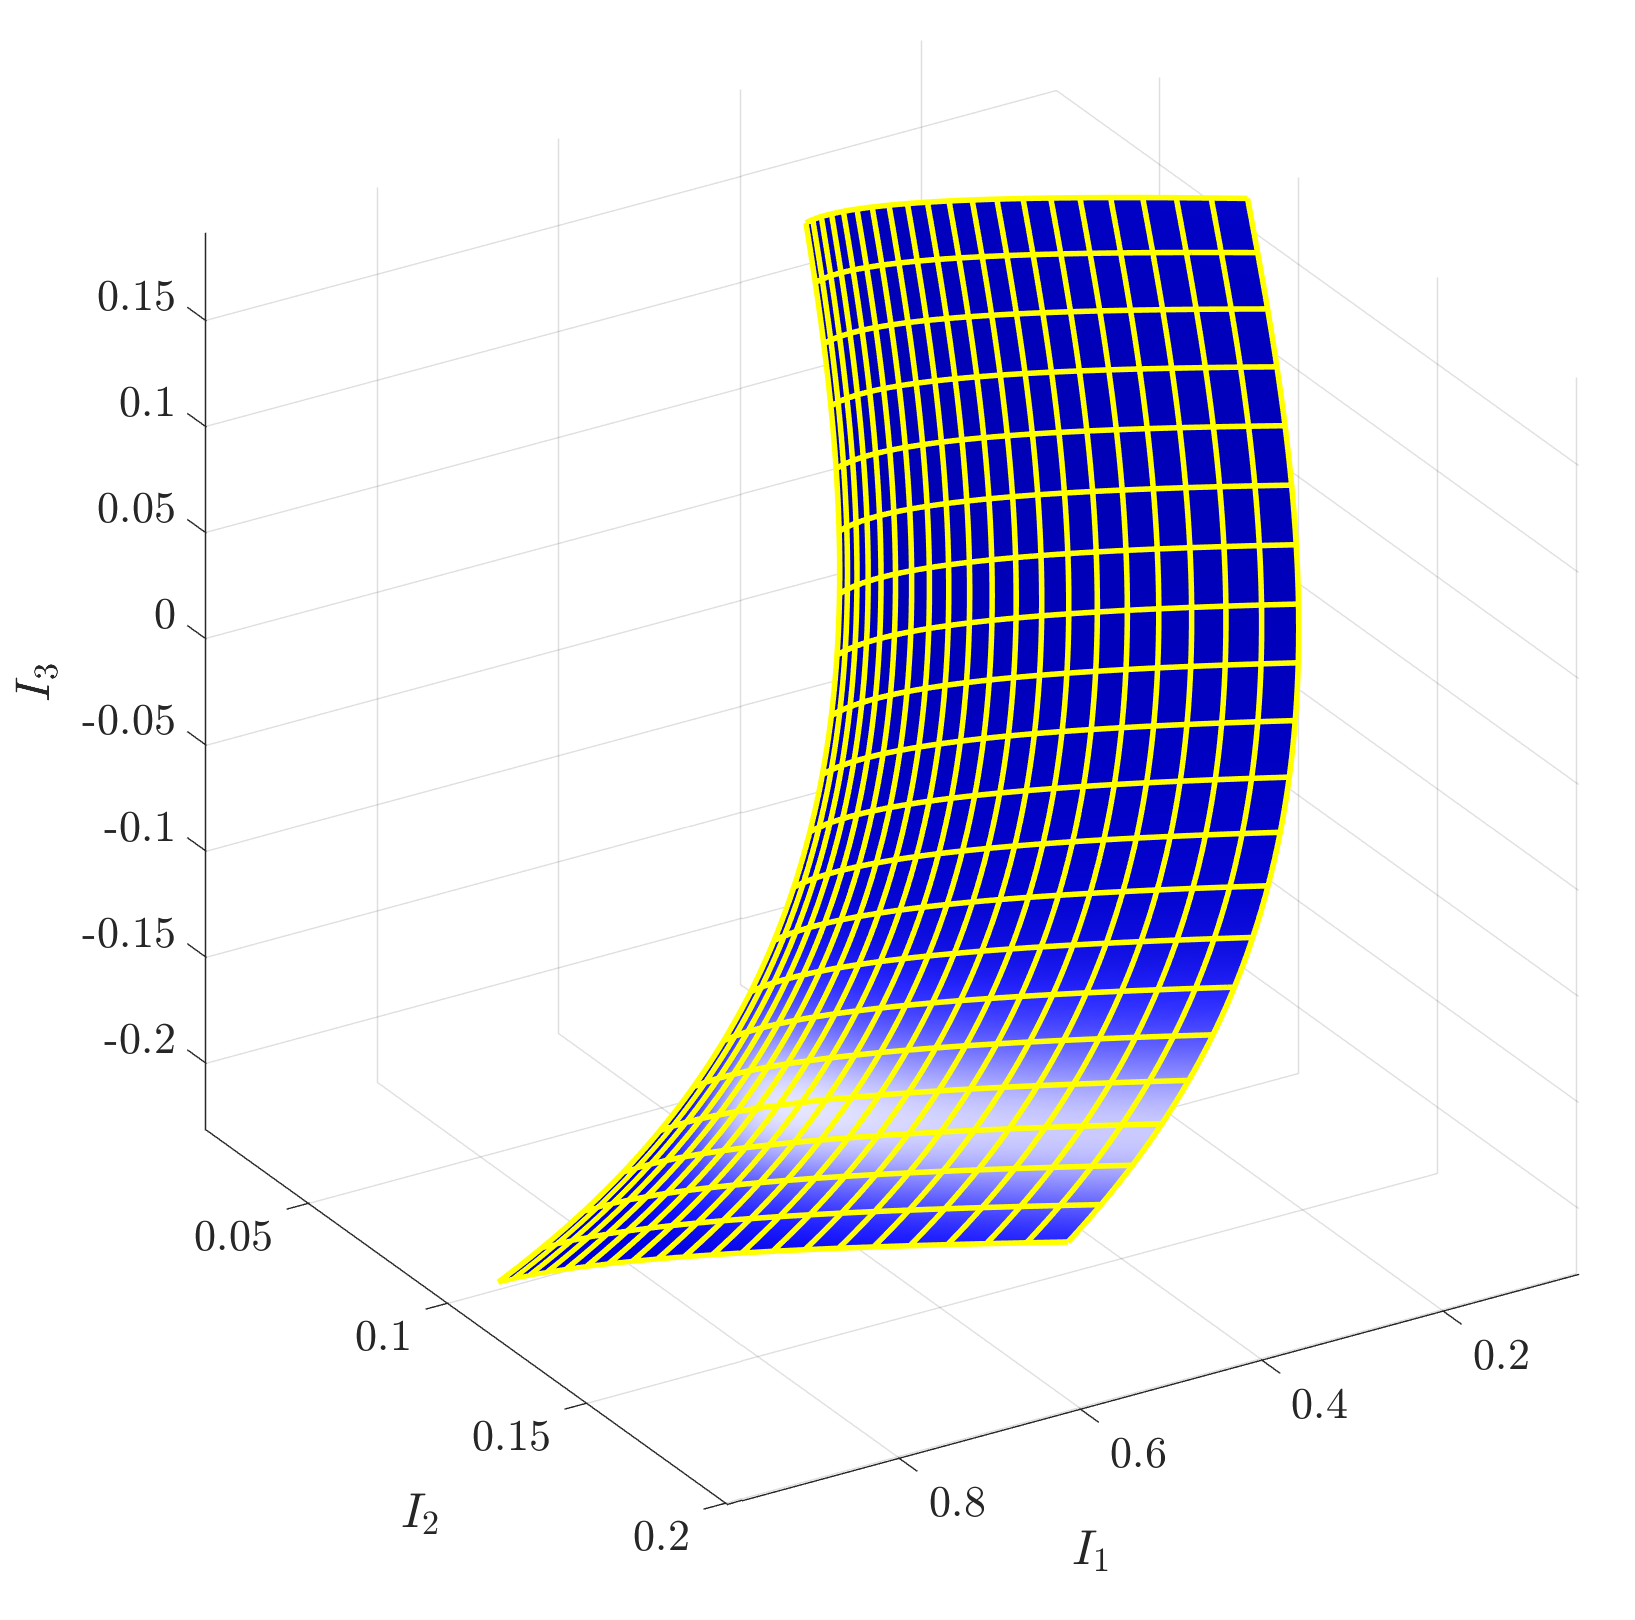
\includegraphics[width=12cm]{figures/E2_signature}
  \caption{$E(2)$ signature}
  \label{fig:e2signature}
\end{figure}

\subsection{SA(2)}
For $SA(2)$, we use the signature
\begin{equation}\label{eq:sa2sig}
  \begin{split}
    I_1 &= f_{xx}f_{yy} - f_{xy}^2  \\
    I_2 &= f_y^2f_{xx} - 2f_x f_y f_{xy} + f_x^2f_{yy} \\
    I_3 &= f_{xxx}f_y^3 - 3*f_{xxy}f_x f_y^2 + 3f_{xyy}f_x^2f_y - f_{yyy}f_x^3
  \end{split}
\end{equation}
The signature is visualised in Fig.~\ref{fig:sa2signature}
\begin{figure}
  \centering
    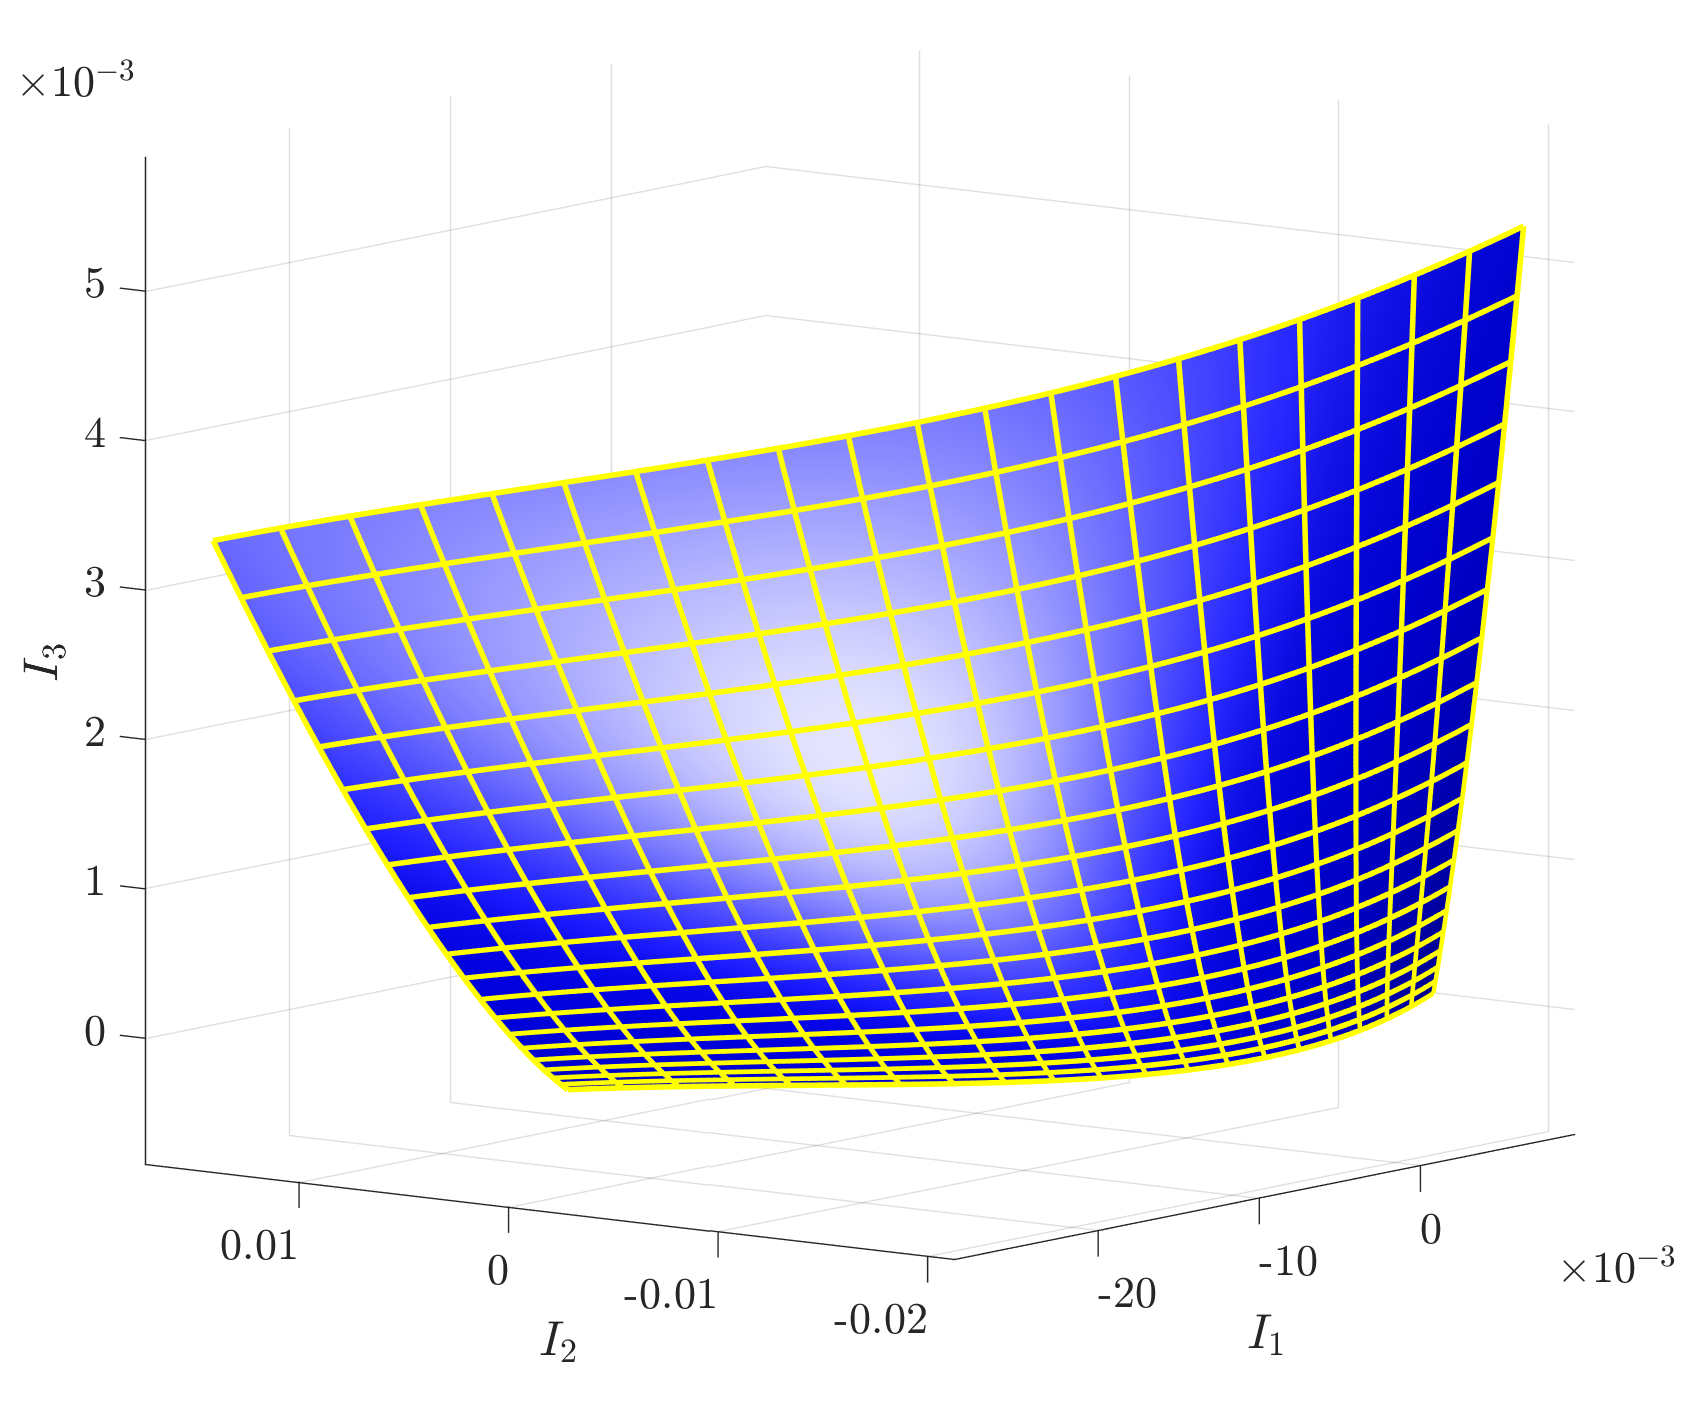
\includegraphics[width=12cm]{figures/SA2_signature}
  \caption{$SA(2)$ signature}
  \label{fig:sa2signature}
\end{figure}

\subsection{A(2)}
For $A(2)$, we use the signature
\begin{equation}\label{eq:a2sig}
  \begin{split}
    I_1 &= \frac{fC^3}{\sqrt{C^6 + D^6 + E^4}} \\
    I_2 &= \frac{fD^3}{\sqrt{C^6 + D^6 + E^4}} \\
    I_3 &= \frac{fE^2}{\sqrt{C^6 + D^6 + E^4}} \\
  \end{split}
\end{equation}
where
\begin{equation*}
  \begin{split}
    C &= f_{xx}f_{yy} - f_{xy}^2 \\
    D &= f_y^2f_{xx} - 2f_xf_y f_{xy} + f_x^2f_{yy} \\
    E &= f_{xxx}f_y^3 - 3f_{xxy}f_x f_y^2 + 3f_{xyy}f_x^2 f_y - f_{yyy}f_x^3
  \end{split}
\end{equation*}
The signature is visualised in Fig.~\ref{fig:a2signature}
\begin{figure}
  \centering
    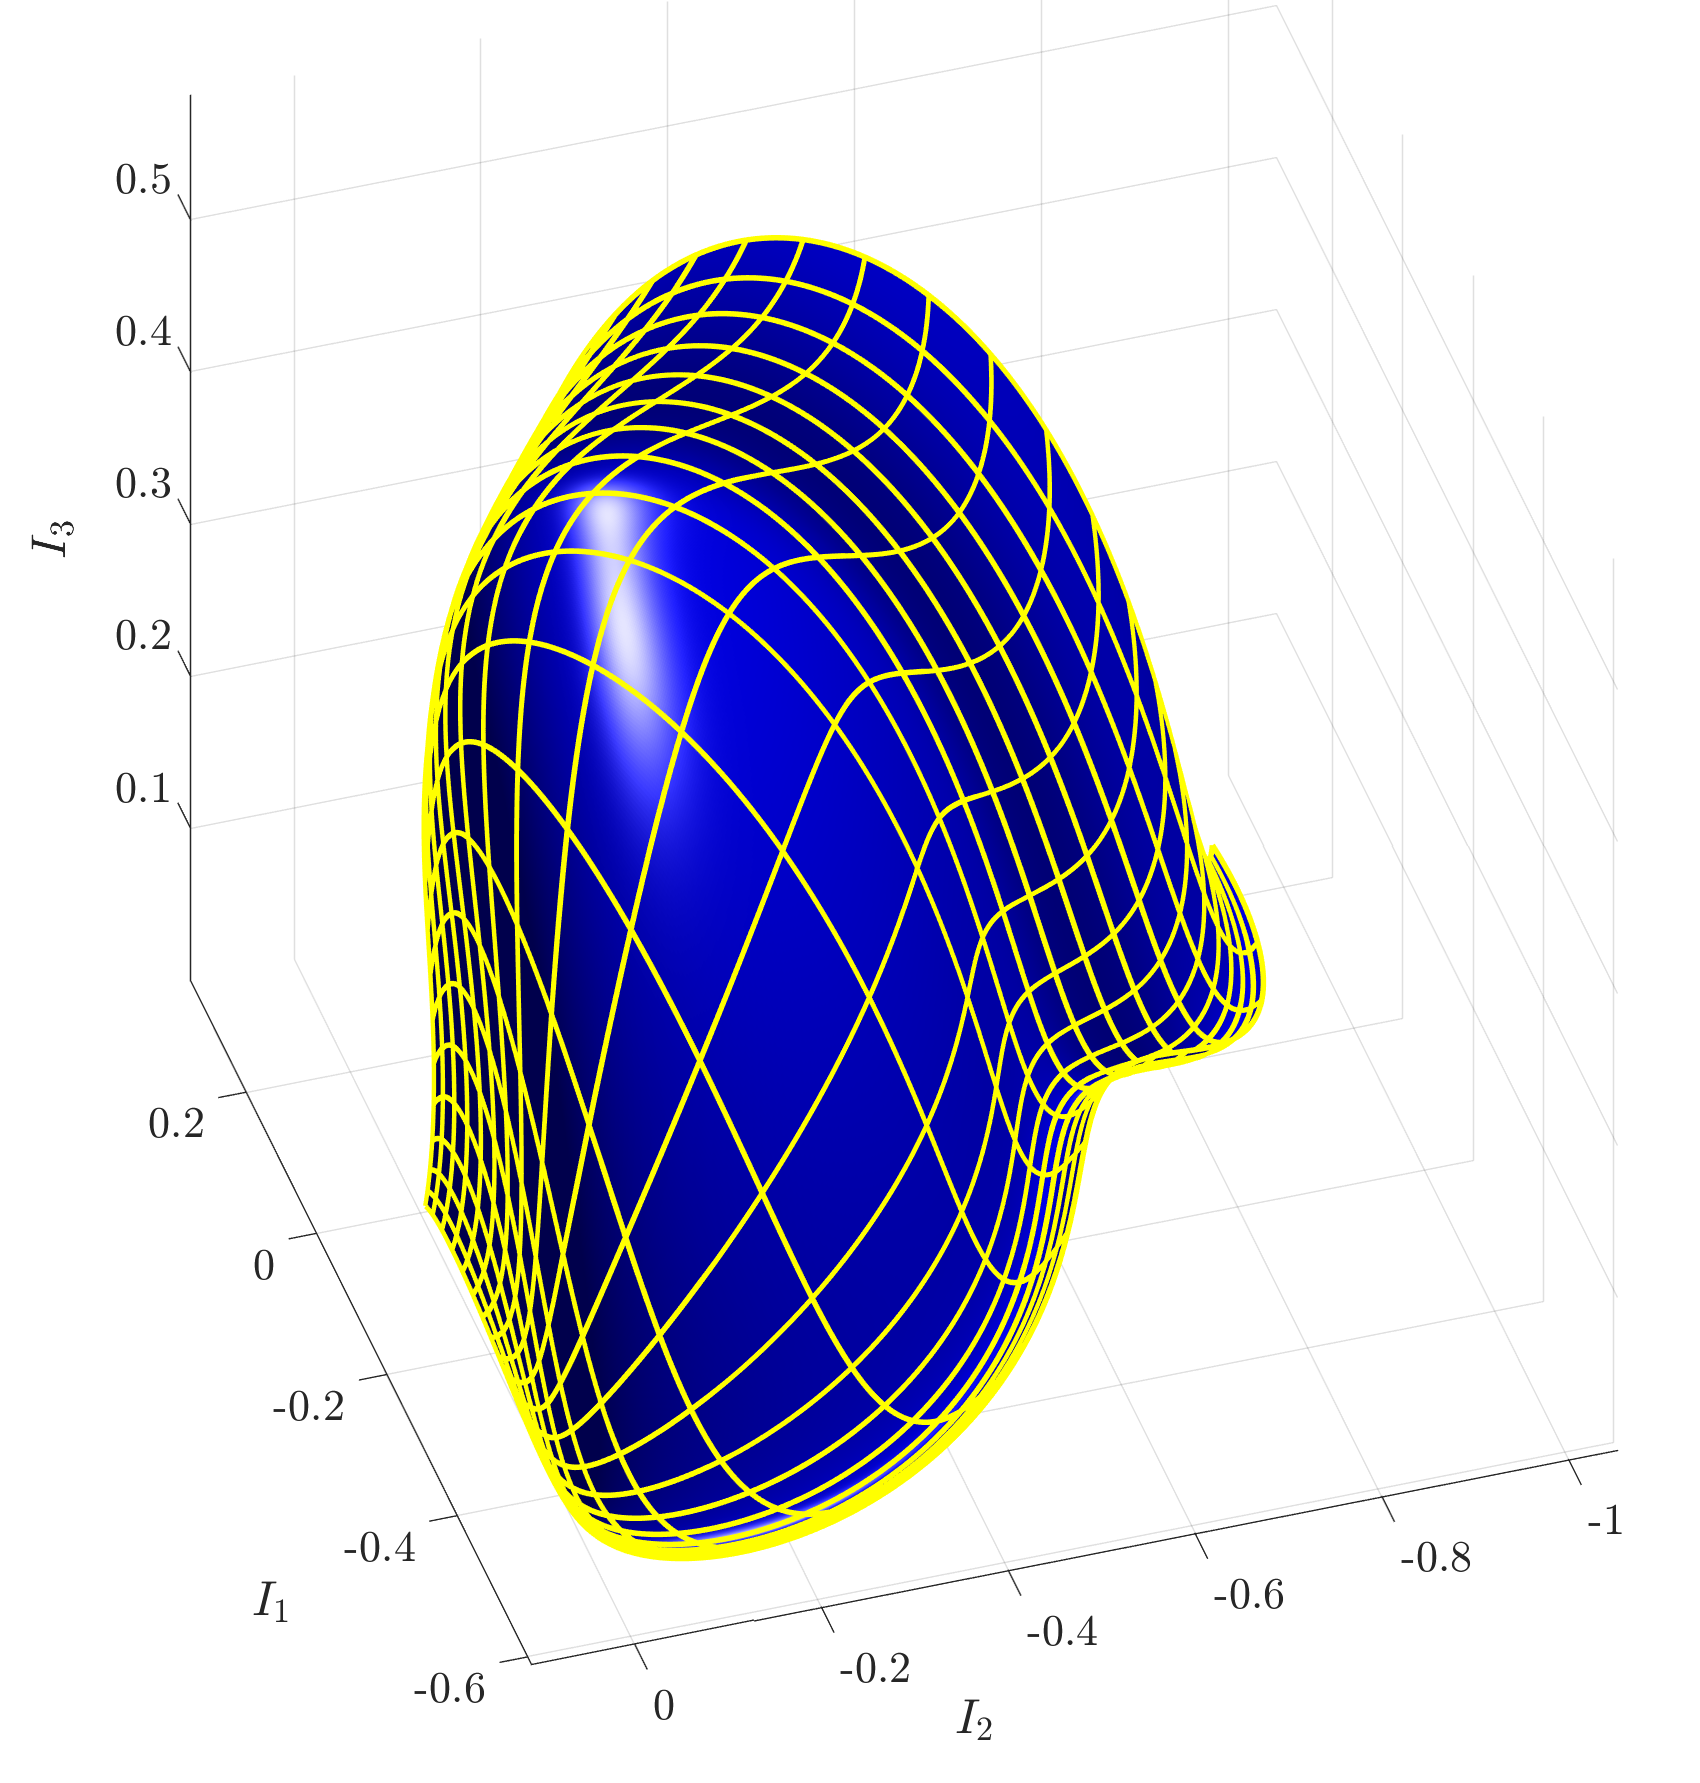
\includegraphics[width=12cm]{figures/A2_signature}
  \caption{$A(2)$ signature}
  \label{fig:a2signature}
\end{figure}

\subsection{M{\"o}bius}
For $\text{M{\"o}bius}$, we use the signature
\begin{equation}\label{eq:mobiussig}
  \begin{split}
    I_1 &= \frac{fJ_1^4}{\sqrt{J_1^8 + K_1^2 + K_4^2}} \\
    I_2 &= \frac{fK_1}{\sqrt{J_1^8 + K_1^2 + K_4^2}} \\
    I_3 &= \frac{fK_4}{\sqrt{J_1^8 + K_1^2 + K_4^2}}
  \end{split}
\end{equation}
where
\begin{equation*}
  \begin{split}
  J_1 &= f_xf_x + f_yf_y \\
  J_2 &= f_{xx} + f_{yy} \\
  J_3 &= J_1(f_x(f_{xxx} + f_{xyy}) + f_y(f_{xxy} + f_{yyy})) + 
      2J_2(f_x^2f_{xx} + 2f_xf_yf_{xy} + f_y^2f_{yy}) \\
  J_4 &= J_1(f_x(f_{xxy} + f_{yyy}) - f_y(f_{xxx} + f_{xyy})) + 
      2J_2(f_x^2f_{xy} + f_xf_yf_{yy} - f_xf_yf_{xx} - f_y^2f_{xy}) \\
  K_1 &= f_y^5f_{yyy} + 9/2f_y^2f_{yy}^2f_x^2 + f_y^3f_{yyy}f_x^2 + 
      3/2f_{yy}^2f_x^4 -9f_y^3f_{yy}f_xf_{xy} + 3f_yf_{yy}f_x^3f_{xy} + \\
      & 3/2f_y^4f_{xy}^2 - 9f_y^2f_x^2f_{xy}^2 + 
      3/2f_x^4f_{xy}^2 + 3f_y^4f_xf_{xyy} + 3f_y^2f_x^3f_{xyy} + \\
      & 3f_y^4f_{yy}f_{xx} + 3f_{yy}f_x^4f_{xx} + 3f_y^3f_xf_{xy}f_{xx} -
      9f_yf_x^3f_{xy}f_{xx} + 3/2f_y^4f_{xx}^2 + 9/2f_y^2f_x^2f_{xx}^2 + \\
      & 3f_y^3f_x^2f_{xxy} + 3f_yf_x^4f_{xxy} + f_y^2f_x^3f_{xxx} + 
      f_x^5f_{xxx} \\
  K_4 &= -3f_yf_{yy}^2f_x^3 + f_y^2f_{yyy}f_x^3 + f_{yyy}f_x^5 +
  9f_y^2f_{yy}f_x^2f_{xy}   - 3f_{yy}f_x^4f_{xy} - 6f_y^3f_xf_{xy}^2 + \\
  & 6f_yf_x^3f_{xy}^2 -   3f_y^3f_x^2f_{xyy} - 3f_yf_x^4f_{xyy} - 
  3f_y^3f_{yy}f_xf_{xx} +   3f_yf_{yy}f_x^3f_{xx} + 3f_y^4f_{xy}f_{xx} -
  \\
  & 9f_y^2f_x^2f_{xy}f_{xx} + 3f_y^3f_xf_{xx}^2 + 3f_y^4f_xf_{xxy} +
  3f_y^2f_x^3f_{xxy} - f_y^5f_{xxx} - f_y^3f_x^2f_{xxx} \\
\end{split}
\end{equation*}
The signature is visualised in Fig.~\ref{fig:mobiussignature}
\begin{figure}
  \centering
    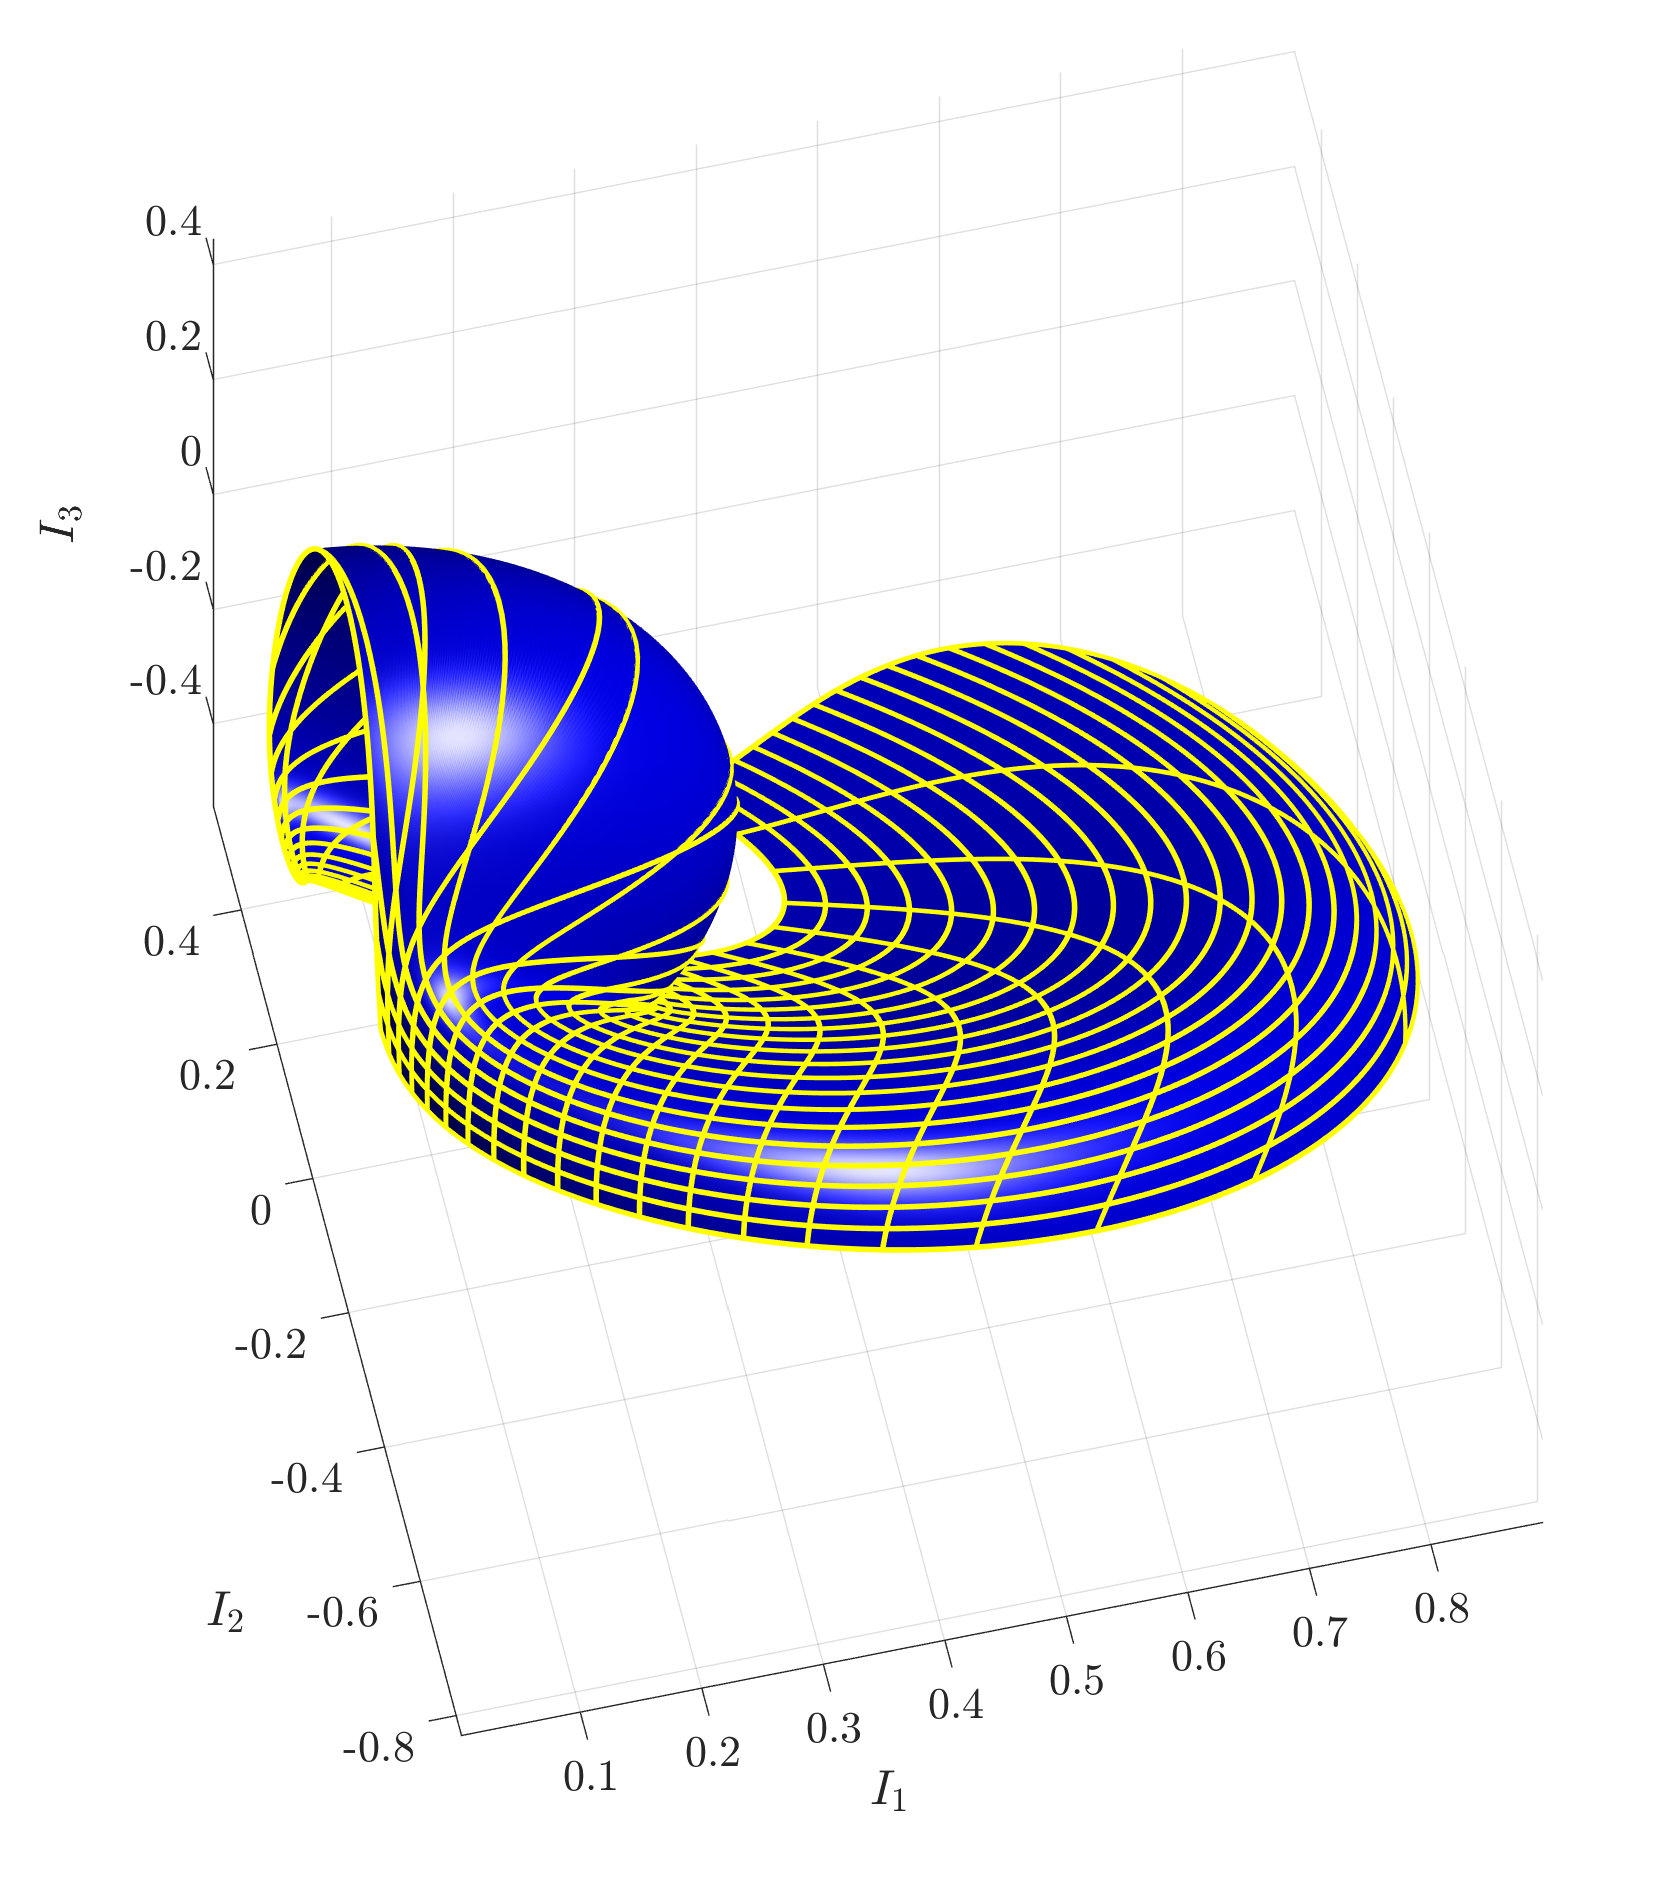
\includegraphics[width=12cm]{figures/Mobius_signature}
    \caption{$\text{M{\"o}bius}$ signature}
  \label{fig:mobiussignature}
\end{figure}

\subsection{$PSL(3, \mathbb{R})$}
For $PSL(3, \mathbb{R})$, we use the signature
\begin{equation}\label{eq:psl3rsig}
  \begin{split}
    I_1 &= \frac{f}{\gamma}D^6 \\
    I_2 &= \frac{f}{\gamma}P_4^3\\
    I_3 &= \frac{f}{\gamma}(E^2- 12DP_5)^2
  \end{split}
\end{equation}
where
\begin{equation*}
  \begin{split}
    C &= f_{xx}f_{yy} - f_{xy}^2 \\
    D &= f_y^2f_{xx} - 2f_xf_yf_{xy} + f_x^2f_{yy} \\
    E &= f_{xxx}f_y^3 - 3f_{xxy}f_xf_y^2 + 3f_{xyy}f_x^2f_y - f_{yyy}f_x^3
    \\
    \gamma &= \sqrt{D^{12} + P_4^6 + (E^2 - 12DP_5)^4} \\
    Q_4 &= 4f_xf_{xy}^2f_{xyy} - f_x^2f_{xyy}^2 - 2f_{yyy}f_xf_{xy}f_{xx} +
    \\
    & 2f_{yy}f_xf_{xyy}f_{xx} - 6f_yf_{xy}f_{xyy}f_{xx} + \\
    & 2f_yf_{yyy}f_{xx}^2 + f_{yyy}f_x^2f_{xxy} - 6f_{yy}f_xf_{xy}f_{xxy} + \\ 
    & 4f_yf_{xy}^2f_{xxy} + f_yf_xf_{xyy}f_{xxy} + 2f_yf_{yy}f_{xx}f_{xxy} - \\
    & f_y^2f_{xxy}^2 + 2f_{yy}^2f_xf_{xxx} - f_yf_{yyy}f_xf_{xxx} \\
    & -2f_yf_{yy}f_{xy}f_{xxx} + f_y^2f_{xyy}f_{xxx} \\
    P_5 &= f_{yyy}f_x^3f_{xy} - f_{yy}f_x^2f_{xy}^2 + 2f_yf_xf_{xy}^3 - \\
    & f_{yy}f_x^3f_{xyy} - f_yf_x^2f_{xy}f_{xyy} + f_{yy}^2f_x^2f_{xx} - \\
    & f_yf_{yyy}f_x^2f_{xx} - 2f_yf_{yy}f_xf_{xy}f_{xx} - \\
    & f_y^2f_{xy}^2f_{xx} + 2f_y^2f_xf_{xyy}f_{xx} + f_y^2f_{yy}f_{xx}^2 + \\
    & 2f_yf_{yy}f_x^2f_{xxy} - f_y^2f_xf_{xy}f_{xxy} - f_y^3f_{xx}f_{xxy} - \\
    & f_y^2f_{yy}f_xf_{xxx} + f_y^3f_{xy}f_{xxx} \\
    P_4 &= -4C^2 + Q_4 
  \end{split}
\end{equation*}
The signature is visualised in Fig.~\ref{fig:psl3rsignature}
\begin{figure}
  \centering
    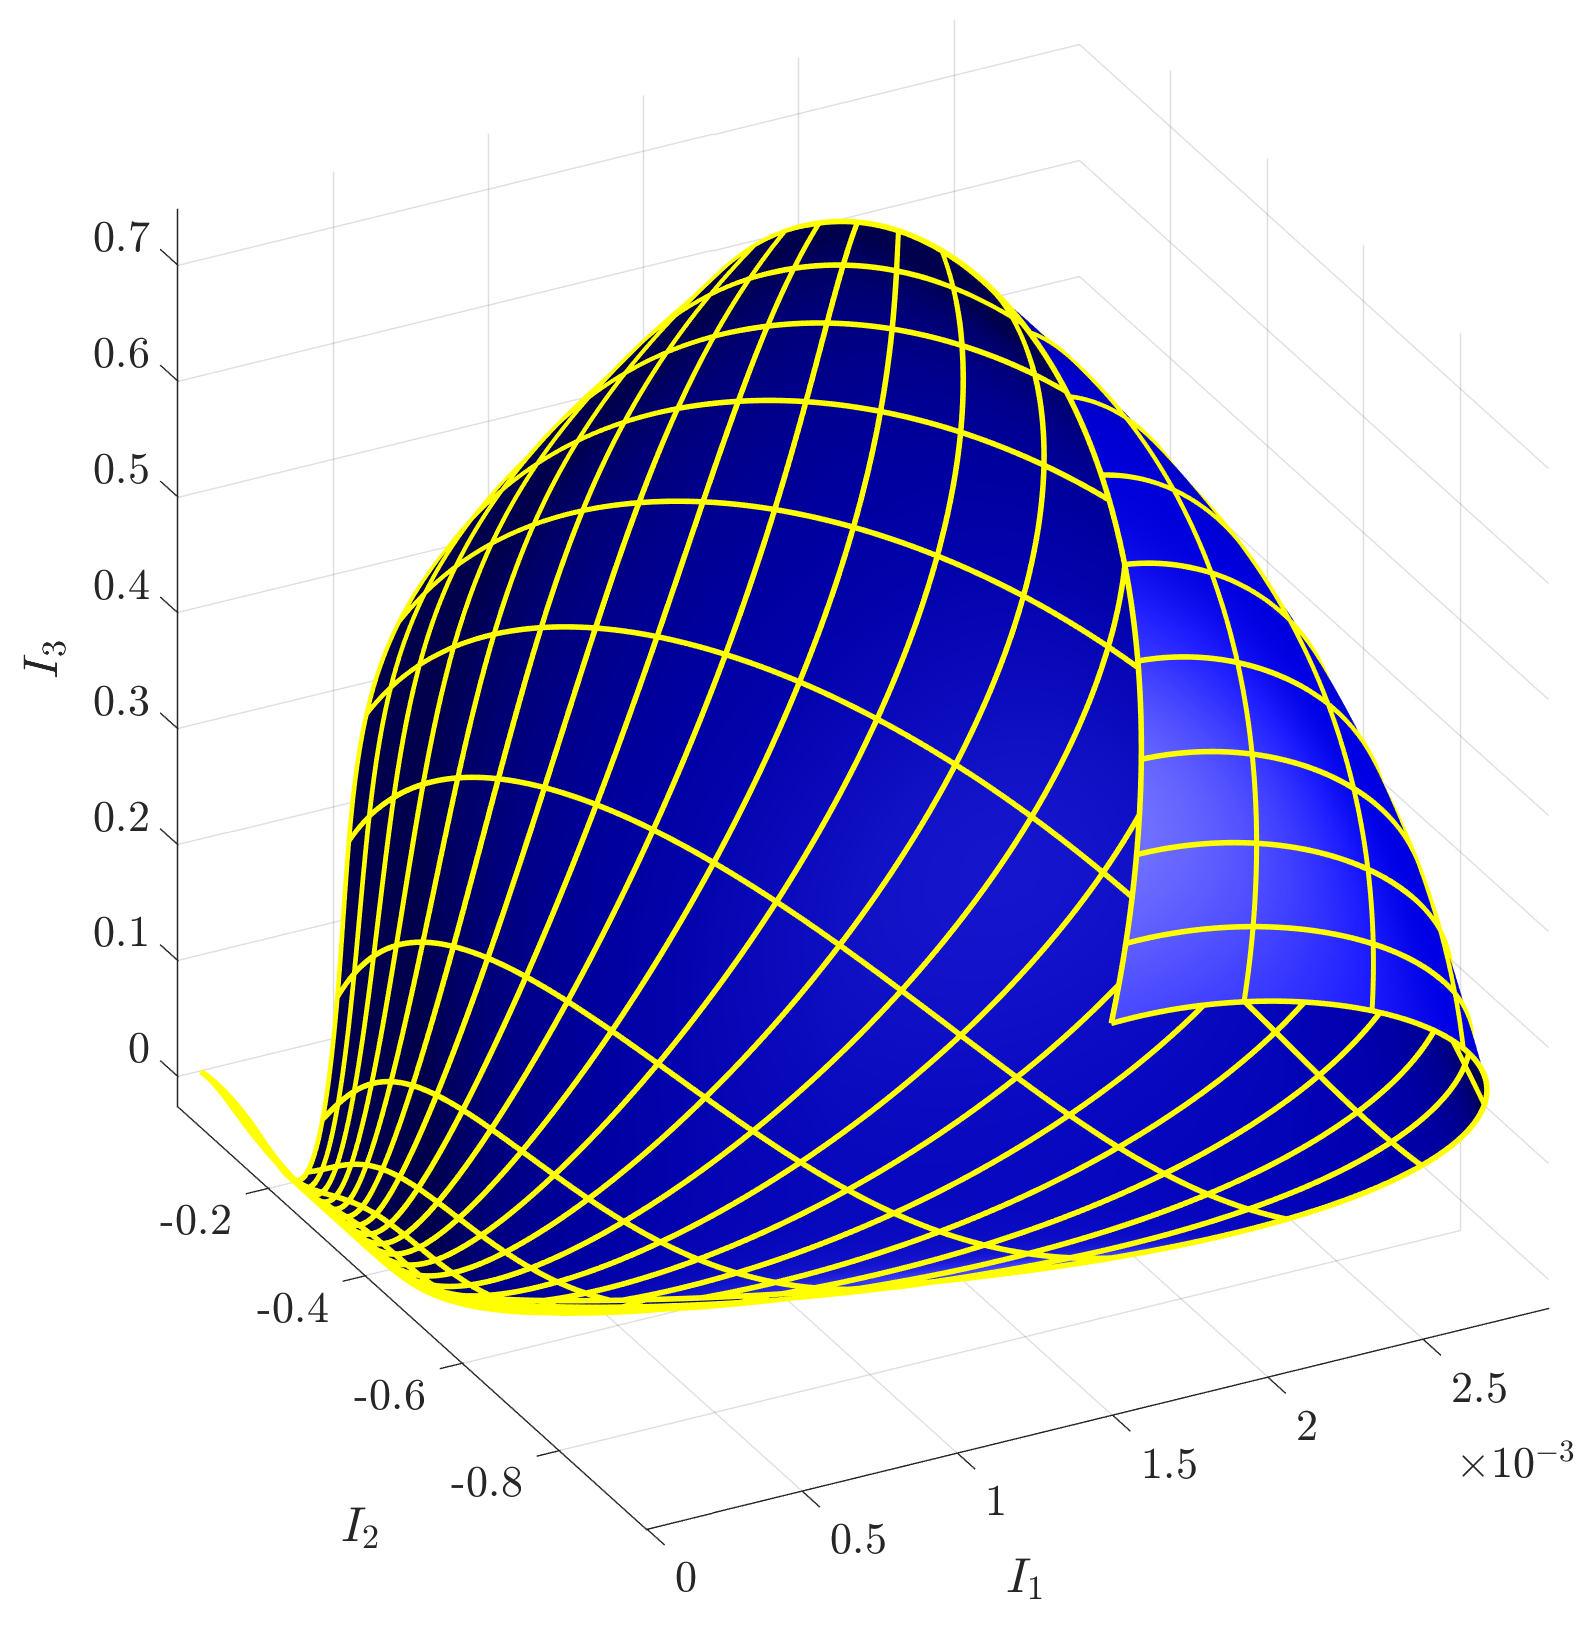
\includegraphics[width=12cm]{figures/PSL3R_signature}
    \caption{$PSL(3, \mathbb{R})$ signature}
  \label{fig:psl3rsignature}
\end{figure}
\end{document}


